\begin{abstract}
Maintaining the diversity in the results of heuristic search has been an
important requirement in the applications of automated planning such as
Penetrating Testing. Also, several inadmissible algorithms incorpolating
diversity are shown to outperform those without it. However, currently,
little has been investigated on the role of diversity in the admissible
search algorithms like A*. 

In this paper, we propose two novel diversified tie-breaking strategies
for A*. The first one is a portfolio-based approach which alternates
between the different expansion strategy like LIFO, FIFO within the same
f-value, while caching the f-value to avoid the costly heuristic
computation. We provide a theoretical worst case guarantee of the number
of heuristic evaluation, and empirically show that the actual
performance is better than the worst case.  The second strategy called
OpenTrees replaces the common bucket-based open list with a tree-based
open list in order to maximize the surprize encountered by expanding the
next node. Both methods preserve the expansion ordering in terms of
f-value, thus maintaining the optimality of the solution.
\end{abstract}

In the applications of automated planning such as Penetrating Testing,
Propositional Planners try to find an attack plan to take control over
the simulated corpolate network, mimicking the behavior of the real
attacker, until the network security is improved and no attack plan
exists \cite{boddy2005course}.  Here, maintaining the diversity of the
attack plans is an important demand by the customers because such
diversity provides a broader insight on the weakness of the corporation
network. To meet these demands, several diversity metrics were
developped \cite{roberts2014evaluating,goldman2015measuring} along with
several algorithms that returns a set of diverse plans
\cite{srivastava2007domain,coman2011generating,nguyen2012generating}.

Diversity, or more frequently referred to as the problem of
\emph{exploration} versus \emph{exploitation}, was also considered
beneficial in improving the search efficiency.  \emph{k-Best First
Search} \cite{felner2003kbfs} and \emph{Diverse Best First Search(DBFS)}
\cite{imai2011novel} were developed for improving the search behavior of
Greedy Best First Search by shifting the balance slightly from
exploitation to exploration, because GBFS is sometimes misdirected by
the errors in the heuristic estimates, and stays too narrowly focused on
the wrong direction.

In Robotics, RRT (Rapidly-exploring Random Tree) algorithm
\cite{lavalle2001randomized} is a \sota randomized algorithm for
high-dimensional, \emph{continuous} space and is widely known for its
provably good balance between exploration and exploitation. Unlike
\astar, this algorithm is not guided at all, i.e.\ it does not use any
heuristic functions, although there are various attempts to implement it
\cite{urmson2003approaches,urmson2003approaches}. Hence several papers
\cite{alcazar2011adapting,burfoot2006rrt,likhachev2008r} have tried to
merge RRT-based algorithms to \astar, which is designed for discrete
state spaces.
%  They wrapped a guided % search with randomized tree construction which allows the planner to search the state space scarcely, and its scarceness has a significant mathematically good characteristics such as uniform distribution and convergence.

Despite these interests, the role of diversity in \(A^*\)-based search
algorithms is underinvestigated.
KBFS, DBFS and GBFS are all inadmissible.
% RRT-based planners do not significantly improve upon the current
% state-of-the-art planner such as LAMA \cite{alcazar2011adapting}, although it
% has improved in some domains.
RRT-based planners are also subjective to the probabilistic convergence,
which means the optimality is guaranteed only when an infinite amount of
search time is provided, or they simply succumb to inadmissible search.


The contribution of this paper is to add a new variety of improvements
to the admissible search techniques.  Recent work by Helmert and Roger
\shortcite{helmert2008good} claims that, even with an optimistic
assumption of \emph{almost-perfect heuristics}, \astar still has an
exponentially large plateau. They conclude that the further performance
improvement requires the techniques orthogonal to the heuristic
function, such as symmetry breaking, domain reduction, factored planning
etc.  Our diversity-based technique falls into this category.

This paper is organized as follows: The next section describes the
background and preliminaries on the theoretical aspects of
\astar. Next, we describe the details of our diversified tie-breaking
method and its theoretical implications.  Then we provide an empirical
result of our algorithm compared to traditional \astar with various
heuristics. We finally conclude with a discussion on the future work.

\section{Backgrounds and Preliminary}
\label{sec-1}

\subsubparagraph{\astar and perfect heuristics}

\astar is a state of the art algorithm for finding an optimal path in the
search space represented as a graph. 
\astar always returns an optimal solution when the heuristic function $h$ is
admissible, i.e., when it never overestimate the true distance to the goal
$h^*$.
% , and the nodes are first ordered according to $f$
% 
Thus, the best possible admissible heuristic function is $h^*$ itself, which is
called \emph{perfect heuristics}. However, computing $h^*$ is PSPACE-Complete,
which is as difficult as solving the problem itself and is not
practical.

%It is known that with a perfect heuristics the planner do not have to
% conduct any search: There are no multiple possibilities that the
% planner should examine on each node.

\emph{Almost perfect} heuristic function $h_c$ is a class of similar
impractical, theoretical functions which is also PSPACE-Complete to
compute \cite{helmert2008good}.  It has a constant error $c$ from the
perfect heuristic $h^*$, i.e., $h_c=h^*-c$.  The important finding by
\citeauthor{helmert2008good} is that even with this intractable and
impractical heuristic function, the number of the nodes in the last
plateau of the search becomes exponentially large as the problem size
increases.  Using this fact, they showed that relying only on the
improvement of the heuristic functions is not fruitful in the near
future, and the researchers should seek the other,
orthorgonal improvement.

These intractable heuristics are of course very hard and expensive to
compute. However, even the practical, tractable heuristic functions
which can be computed in polynomial time, such as \lmcut and M\&S, are
also very computationally expensive. Compared to the other functions,
these functions dominate the search time over the other factors of
planning algorithms, such as node insertion and deletion.

\section{Tie Breaking Criteria in \astar}

% Compared to the other algorithms which
% guarantee optimality such as $IDA^*$ \cite{korf1985depth}, \astar requires a large amount of % memory to store the search nodes.

\astar stores the search nodes into two priority queues called an \emph{open list} and a \emph{closed list}, sorted based on $f$ value. While the implementation of the priority queue varies, it has another degree of freedom called tie-breaking, i.e. how to select the next node to open within the same priority.

In the current implementation of the \sota admissible planning systen Fast Downward (FD) \cite{Helmert2006}, the standard \astar search breaks ties based on $h$, meaning that if two nodes have the same $f$ value, the nodes with smaller $h$ will be selected, in other words favoring the nodes with larger $g$ values (since $f=g+h$). The intension behind this is that the $h$ values are just an \emph{estimate} to the goal, while $g$ values are the \emph{actual} distance from the initial state and more reliable.

Another thing we have to note is that in FD, when even the $h$ values are the same, then the second tiebreaking behavior is basically a FIFO order: The planner selects the nodes that is inserted earlier. 

However, in fact, these tiebreaking methods are not necessary when we are only concerned with  maintaining the optimality. These tiebreaking criteria are just the result of heuristic, ad-hoc selection by humans and have no theoretical background.
% In particular, we first observed that this FIFO order has not legitimate reason to support.

We therefore ran a preliminary experiments on various benchmark domains, comparing a simple FIFO-order, LIFO-order and Random order using 5 minutes runtime cutoff. 
All experiments below are conducted on a cluster with Xeon E5410@2.33GHz CPUs.
We observed that even such a slightest difference can change the performance significantly, depending on the domains.
\refig{single-eval} compares the number of node evaluation (computations of \lmcut)
by LIFO, FIFO and Random second tiebreaking.
According to the figure, LIFO has smaller number of evaluations than the others in Openstacks, but Random dominates the others in Miconic and Nomystery, indicating that there are no dominance relationship between these three.
\reftbl{single-coverage} shows the coverage result (number of problems solved) by each strategy.
Overall, LIFO strategy achieved a higher coverage.

Note that, although LIFO dominated the others, we consider this is just by a coincidence due to our selection of problems, time limit and domains. we \emph{are not trying to claim that any of LIFO or FIFO or Random order dominates the other}. However, there are noticeable performance difference cause by these different tiebreaking strategies.

\begin{figure}[htbp]
 \centering
 \relsize{-2}
 \includegraphics{tables/aaai16-evaluated-lmcut_ff-lmcut_r.pdf}
 \includegraphics{tables/opt11-evaluated-lmcut_ff-lmcut_lf.pdf}
 \includegraphics{tables/opt11-evaluated-lmcut_lf-lmcut_r.pdf}
\caption{Comparison of the number of node evaluations (computations of \lmcut) by FIFO and LIFO tie breaking, on IPC2011 optimal track instance. LIFO order dominates FIFO and Random order especially in openstacks instances, and the gap is more than one the order of 10.}
 \label{single-eval}
\end{figure}

\begin{table}[htbp]
 \centering
 \relsize{-2}
 \begin{tabular}{|c|c|c||c||c||c||c||c||c||c|}
   \hline                        
   &  Domain & \rotatebox[origin=l]{0}{${\mbox{lmcut}}_{\mbox{ffff1}}$}   & \rotatebox[origin=l]{0}{${\mbox{lmcut}}_{\mbox{ff1}}$}   & \rotatebox[origin=l]{0}{${\mbox{lmcut}}_{\mbox{lf1}}$}   & \rotatebox[origin=l]{0}{${\mbox{lmcut}}_{\mbox{r1}}$}   & \rotatebox[origin=l]{0}{${\mbox{lmcut}}_{\mbox{fflf1}}$}   & \rotatebox[origin=l]{0}{${\mbox{lmcut}}_{\mbox{ffr1}}$}   & \rotatebox[origin=l]{0}{${\mbox{lmcut}}_{\mbox{lfr1}}$}   & \rotatebox[origin=l]{0}{${\mbox{lmcut}}_{\mbox{fflfr1}}$}    \\
   \hline                        
\multirow{45}{*}{\rotatebox[origin=c]{90}{}}   &  {\relsize{-1}airport(50)} &  \textbf{28} &  \textbf{28} &  27 &  27 &  \textbf{28} &  \textbf{28} &  27 &  \textbf{28}  \\
   &  {\relsize{-1}barman-opt11-strips(20)} &  \textbf{4} &  \textbf{4} &  \textbf{4} &  3 &  \textbf{4} &  \textbf{4} &  \textbf{4} &  \textbf{4}  \\
   &  {\relsize{-1}blocks(136)} &  24 &  24 &  \textbf{26} &  25 &  \textbf{26} &  \textbf{26} &  \textbf{26} &  \textbf{26}  \\
   &  {\relsize{-1}blocks-3op(30)} &  \textbf{10} &  \textbf{10} &  \textbf{10} &  \textbf{10} &  \textbf{10} &  \textbf{10} &  \textbf{10} &  \textbf{10}  \\
   &  {\relsize{-1}childsnack-opt14-strips(20)} &  \textbf{0} &  \textbf{0} &  \textbf{0} &  \textbf{0} &  \textbf{0} &  \textbf{0} &  \textbf{0} &  \textbf{0}  \\
   &  {\relsize{-1}cybersec(19)} &  2 &  2 &  3 &  \textbf{9} &  3 &  \textbf{9} &  8 &  8  \\
   &  {\relsize{-1}depot(22)} &  \textbf{7} &  \textbf{7} &  \textbf{7} &  \textbf{7} &  6 &  6 &  \textbf{7} &  \textbf{7}  \\
   &  {\relsize{-1}driverlog(20)} &  \textbf{13} &  \textbf{13} &  \textbf{13} &  \textbf{13} &  \textbf{13} &  \textbf{13} &  \textbf{13} &  \textbf{13}  \\
   &  {\relsize{-1}elevators-opt11-strips(20)} &  \textbf{17} &  \textbf{17} &  16 &  16 &  15 &  14 &  14 &  14  \\
   &  {\relsize{-1}ferry(30)} &  \textbf{30} &  \textbf{30} &  \textbf{30} &  \textbf{30} &  \textbf{30} &  \textbf{30} &  \textbf{30} &  \textbf{30}  \\
   &  {\relsize{-1}floortile-opt11-strips(20)} &  \textbf{6} &  \textbf{6} &  \textbf{6} &  \textbf{6} &  \textbf{6} &  \textbf{6} &  \textbf{6} &  \textbf{6}  \\
   &  {\relsize{-1}freecell(80)} &  \textbf{13} &  \textbf{13} &  12 &  \textbf{13} &  \textbf{13} &  \textbf{13} &  \textbf{13} &  \textbf{13}  \\
   &  {\relsize{-1}ged-opt14-strips(20)} &  \textbf{15} &  \textbf{15} &  \textbf{15} &  \textbf{15} &  \textbf{15} &  \textbf{15} &  \textbf{15} &  13  \\
   &  {\relsize{-1}grid(5)} &  \textbf{2} &  \textbf{2} &  \textbf{2} &  \textbf{2} &  \textbf{2} &  \textbf{2} &  \textbf{2} &  \textbf{2}  \\
   &  {\relsize{-1}gripper(20)} &  \textbf{6} &  \textbf{6} &  \textbf{6} &  \textbf{6} &  \textbf{6} &  \textbf{6} &  \textbf{6} &  \textbf{6}  \\
   &  {\relsize{-1}hanoi(30)} &  \textbf{12} &  \textbf{12} &  \textbf{12} &  \textbf{12} &  \textbf{12} &  11 &  \textbf{12} &  \textbf{12}  \\
   &  {\relsize{-1}hiking-opt14-strips(20)} &  \textbf{8} &  \textbf{8} &  \textbf{8} &  \textbf{8} &  \textbf{8} &  \textbf{8} &  \textbf{8} &  \textbf{8}  \\
   &  {\relsize{-1}logistics00(199)} &  \textbf{21} &  \textbf{21} &  20 &  \textbf{21} &  \textbf{21} &  \textbf{21} &  20 &  \textbf{21}  \\
   &  {\relsize{-1}maintenance-opt14-adl(5)} &  \textbf{5} &  \textbf{5} &  \textbf{5} &  \textbf{5} &  \textbf{5} &  \textbf{5} &  \textbf{5} &  \textbf{5}  \\
   &  {\relsize{-1}miconic(150)} &  \textbf{140} &  \textbf{140} &  \textbf{140} &  \textbf{140} &  \textbf{140} &  \textbf{140} &  \textbf{140} &  \textbf{140}  \\
   &  {\relsize{-1}movie(30)} &  \textbf{30} &  \textbf{30} &  \textbf{30} &  \textbf{30} &  \textbf{30} &  \textbf{30} &  \textbf{30} &  \textbf{30}  \\
   &  {\relsize{-1}mprime(35)} &  \textbf{22} &  \textbf{22} &  \textbf{22} &  \textbf{22} &  \textbf{22} &  21 &  \textbf{22} &  \textbf{22}  \\
   &  {\relsize{-1}mystery(30)} &  16 &  16 &  \textbf{17} &  16 &  \textbf{17} &  16 &  16 &  \textbf{17}  \\
   &  {\relsize{-1}no-mprime(35)} &  \textbf{22} &  \textbf{22} &  \textbf{22} &  \textbf{22} &  \textbf{22} &  \textbf{22} &  \textbf{22} &  \textbf{22}  \\
   &  {\relsize{-1}nomystery-opt11-strips(20)} &  \textbf{14} &  \textbf{14} &  \textbf{14} &  \textbf{14} &  \textbf{14} &  \textbf{14} &  \textbf{14} &  \textbf{14}  \\
   &  {\relsize{-1}openstacks-opt11-strips(20)} &  11 &  11 &  \textbf{19} &  10 &  18 &  10 &  16 &  16  \\
   &  {\relsize{-1}parcprinter-opt11-strips(20)} &  \textbf{13} &  \textbf{13} &  \textbf{13} &  \textbf{13} &  \textbf{13} &  \textbf{13} &  \textbf{13} &  \textbf{13}  \\
   &  {\relsize{-1}parking-opt11-strips(20)} &  \textbf{1} &  \textbf{1} &  \textbf{1} &  \textbf{1} &  \textbf{1} &  \textbf{1} &  \textbf{1} &  \textbf{1}  \\
   &  {\relsize{-1}pathways(30)} &  \textbf{5} &  \textbf{5} &  \textbf{5} &  \textbf{5} &  \textbf{5} &  \textbf{5} &  \textbf{5} &  \textbf{5}  \\
   &  {\relsize{-1}pegsol-opt11-strips(20)} &  \textbf{17} &  \textbf{17} &  \textbf{17} &  16 &  \textbf{17} &  16 &  16 &  16  \\
   &  {\relsize{-1}pipesworld-notankage(50)} &  \textbf{16} &  \textbf{16} &  \textbf{16} &  \textbf{16} &  \textbf{16} &  \textbf{16} &  \textbf{16} &  \textbf{16}  \\
   &  {\relsize{-1}pipesworld-tankage(50)} &  \textbf{9} &  8 &  \textbf{9} &  \textbf{9} &  \textbf{9} &  8 &  8 &  8  \\
   &  {\relsize{-1}psr-small(50)} &  \textbf{48} &  \textbf{48} &  \textbf{48} &  \textbf{48} &  \textbf{48} &  \textbf{48} &  \textbf{48} &  \textbf{48}  \\
   &  {\relsize{-1}rovers-large(40)} &  \textbf{7} &  \textbf{7} &  \textbf{7} &  \textbf{7} &  \textbf{7} &  \textbf{7} &  \textbf{7} &  \textbf{7}  \\
   &  {\relsize{-1}scanalyzer-opt11-strips(20)} &  \textbf{9} &  \textbf{9} &  \textbf{9} &  \textbf{9} &  \textbf{9} &  \textbf{9} &  8 &  \textbf{9}  \\
   &  {\relsize{-1}sokoban-opt11-strips(20)} &  19 &  \textbf{20} &  \textbf{20} &  \textbf{20} &  \textbf{20} &  \textbf{20} &  \textbf{20} &  19  \\
   &  {\relsize{-1}storage(30)} &  \textbf{15} &  \textbf{15} &  \textbf{15} &  \textbf{15} &  \textbf{15} &  \textbf{15} &  \textbf{15} &  \textbf{15}  \\
   &  {\relsize{-1}tetris-opt14-strips(17)} &  \textbf{3} &  \textbf{3} &  \textbf{3} &  \textbf{3} &  \textbf{3} &  \textbf{3} &  \textbf{3} &  \textbf{3}  \\
   &  {\relsize{-1}tidybot-opt11-strips(20)} &  \textbf{13} &  \textbf{13} &  \textbf{13} &  \textbf{13} &  \textbf{13} &  \textbf{13} &  \textbf{13} &  \textbf{13}  \\
   &  {\relsize{-1}tpp(30)} &  \textbf{6} &  \textbf{6} &  \textbf{6} &  \textbf{6} &  \textbf{6} &  \textbf{6} &  \textbf{6} &  \textbf{6}  \\
   &  {\relsize{-1}transport-opt11-strips(20)} &  \textbf{6} &  \textbf{6} &  \textbf{6} &  \textbf{6} &  \textbf{6} &  \textbf{6} &  \textbf{6} &  \textbf{6}  \\
   &  {\relsize{-1}tsp(30)} &  \textbf{30} &  \textbf{30} &  \textbf{30} &  \textbf{30} &  \textbf{30} &  \textbf{30} &  \textbf{30} &  \textbf{30}  \\
   &  {\relsize{-1}visitall-opt11-strips(20)} &  \textbf{10} &  \textbf{10} &  \textbf{10} &  \textbf{10} &  \textbf{10} &  \textbf{10} &  \textbf{10} &  \textbf{10}  \\
   &  {\relsize{-1}woodworking-opt11-strips(20)} &  8 &  8 &  \textbf{9} &  8 &  8 &  8 &  8 &  8  \\
   &  {\relsize{-1}zenotravel(20)} &  \textbf{12} &  \textbf{12} &  \textbf{12} &  \textbf{12} &  \textbf{12} &  \textbf{12} &  \textbf{12} &  \textbf{12}  \\
   \hline                        
   &  Sum &  725 &  725 &  \textbf{735} &  729 &  734 &  726 &  731 &  732 \\
\hline
\end{tabular}

 \caption{Preliminary experiments comparing the performance of FIFO, LIFO and Random second-level tiebreaking using Fast Downward. Each cell denotes the problem solved with 5 minutes runtime, 2GB memory limitation. \textbf{Boldface} denotes the case where it achieved the best result among configurations. LIFO tiebreaking was obtained by modifying the TieBreakingOpenList in FD. Both FIFO and LIFO use $[g+h,h]$ as a sorting criteria, where $h=$\lmcut. For Random tiebreaking, we implemented a so-called ``random heuristics'' $r$, which always returns a random value, then used it as the second tiebreaking, i.e., $[g+h,h,r]$. The seed is initialized to 1.}
 \label{single-coverage}
\end{table}

We also observed such differences occur especially in the problems which have the huge search plateau, i.e., the problems where the planner relies heavily on the tiebreaking criteria.  \refig{plateau-h} shows the size of the bucket in a priority queue when the solution is found, compared to the total amount of effort in the search. 
The nodes in a same bucket shares the same $[f,h]$ value, therefore it cannot be guided by the  heuristic functions within this bucket.
Some domains clearly exhibits the large amount of effort is spent on searching through the last plateau, and those domains are greatly affected by the difference in the second tiebreaking such as LIFO, FIFO or Random, according to the previous figures.

In \refig{plateau-h}, we also compared the similar statistics where the $h$-based tiebreaking is disabled. We observed that much higher amount of effort is spent on the plateau based on single-element tiebreaking vector $[f]$.

\begin{figure}[htbp]
 \centering
 \relsize{-2}
 \includegraphics{tables/aaai16-front-vs-evaluated.pdf}
 \caption{Comparison of the size of the search plateau compared to the total evaluation. Data were obtained by the result of standard FIFO tiebreaking on the standard benchmark instances. Both axes are logarithmic. Each dotted line represents 10x, 100x ... lines.  Openstacks,  clearly has the large plateaus.}
 \label{plateau-h}
\end{figure}

\begin{figure}[htbp]
 \centering
 \relsize{-2}
 \includegraphics{tables/aaai16-front-vs-evaluated.pdf}
 \caption{Comparison of the size of the search plateau compared to the total evaluation. Data were obtained by the result of running \astar on the standard benchmark instances, with FIFO but without the tiebreaking by $h$. Both axes are logarithmic. Each dotted line represents 10x, 100x ... lines.}
 \label{plateau-f}
\end{figure}


We can have several important observations from these results.  Firstly, in a plateau, \textbf{the heuristic functions are not used at all, nor the search is guided at all}. This observation holds even if we combine several nondominating heuristics for tie breaking e.g. \lmcut and M\&S.  It is still possible that a plateau is encountered, since their combination is not a perfect heuristics yet!

Secondly, such a plateau is known to be inevitable even if we have an almost perfect heuristics $h_c$, and it is impossible to improve upon $h_c$ --- if it could, the result would be a perfect heuristics or an inadmissible heuristics. Therefore, this problem \textbf{cannot be solved by improving the heuristic accuracy, which is the currently dominating meta-strategy to improve the planner performance.}  Note that combining multiple heuristic functions by taking their maximum is still an attempt to improve the accuracy, therefore it does not solve this problem.

Thirdly, there is no legitimate reason which supports each tiebreaking strategy. \textbf{$h$ and FIFO are just heuristically chosen by the implementer of the planner.} Nor are there any reason to choose LIFO, or Random tie breaking. Notably, it iscan be easily inferred that the different seed value of a Random tiebreaking yield the different search behavior and different result. (In all of our experiment we fixed the seed to 1.)

Based on these observation, the next step we have taken is to develop a new
portfolio-based multi-tiebreaking strategy \textbf{which is orthogonal to
the approach of improving the heuristic accuracy.}

\section{MultiSearch Engine}

We call our new search algorithm within \astar a \emph{MultiSearch}.
It simulates multiple search engines using the same heuristic functions,
but with the different tiebreaking strategies.  Each engine has completely
separate open list and closed list.  However, there is a
globally shared hash table which fully caches the result of heuristic
functions.  Whenever a search engine expands a state, it checks if the
result of a heuristic is already computed, and if yes, it reuses the
result.  Each search engine expands a state in turns, sequencially. The algorithm
finishes when some engine finds the solution.

Assume now we use two \astar engines, both using $f=g+h$ where $h=$\lmcut, both using $h$ as the first tiebreaking, and each using FIFO and LIFO as the second tiebreaking.
The amount of memory used for the open/closed list is doubled, and the effort to push/pop the search nodes is also doubled.
However, the computation of \lmcut is so heavy that those wasted efforts are negligeble.
We first verified this by running a MultiSearch search engine with two same search engines, each using \lmcut and FIFO queue, and compared its runtime agains the single engine using \lmcut and FIFO. The result in \refig{ffff} shows that the extra cost of duplicated effort is negligeble.

\begin{figure}[htbp]
 \centering
 \relsize{-2}
 \includegraphics{tables/opt11-time-lmcut_ff-lmcut_ffff.pdf}
 \caption{Comparison of runtime on problems solved by both single FIFO search engine (ff) and a MultiSearch engine with 2 different instances of the same FIFO engine (ffff). The runtime difference was on average below a factor of x1.1, if we ignore the subsecond differences.}
 \label{ffff}
\end{figure}

This portfolio strategy has several interesting theoretical characteristics. First, if we ignore the negligeble cost of insertion and deletion to the open/closed list, we do not have to pay the extra cost evaluating the heuristic function for states $f<f^*$ thanks to the caching.
Recall that \astar always has to expand the states whose $f$ values are below $f^*$, the true distance from the initial state to the goal. If the heuristic estimate $h$, and in turn $f=g+h$ is the same, any tiebreaking strategy expands and evaluates the same set of nodes in $f<f*$.
Therefore, in region $f<f*$, our caching mechanism fully works and completely eliminates the possibility of extra evaluation caused by adding another queues.

Second, since the search terminates when \emph{some} engine finds a solution, and since the expansion happens in turns, the search effort within the final plateau is upper-bound by \emph{twice} the \emph{minimum} of the search efforts required by LIFO or FIFO engine. This is desirable because, as we saw in the last section, in some domains the gap between the best and worst tiebreaking strategy can be more than 10 times (Openstacks, for example).
When there are $n$ engines, then this increases to $n\times$ minimum amount of effort by each single engine.

Finally, we conducted experiments for evaluating our MultiSearch strategy.
% the number of evaluations and expansions, along with 
\refig{portfolio-ff} to \refig{portfolio-r} shows the runtime between different combinations of 2 or 3 tiebreaking strategies (FIFO+LIFO, FIFO+Random, LIFO+Random, FIFO+LIFO+Random) and the single tiebreaking strategies. The results support our claim that the evaluation never exceeds twice/thirds of the single search engine and, in practice, the evaluations are mostly the same with the single search engine, and in some domains with large plateaus, the search effort used by MultiSearch is more than ten times less than by the single strategy.

\begin{figure}[htbp]
 \centering
 \relsize{-2}
 \includegraphics{tables/opt11-evaluated-lmcut_ff-lmcut_fflf.pdf}
 \includegraphics{tables/opt11-evaluated-lmcut_ff-lmcut_ffr.pdf}
 \includegraphics{tables/opt11-evaluated-lmcut_ff-lmcut_fflfr.pdf}
 \caption{}
 \label{portfolio-ff}
\end{figure}

\begin{figure}[htbp]
 \centering
 \relsize{-2}
 \includegraphics{tables/opt11-evaluated-lmcut_lf-lmcut_fflf.pdf}
 \includegraphics{tables/opt11-evaluated-lmcut_lf-lmcut_lfr.pdf}
 \includegraphics{tables/opt11-evaluated-lmcut_lf-lmcut_fflfr.pdf}
 \caption{}
 \label{portfolio-lf}
\end{figure}

\begin{figure}[htbp]
 \centering
 \relsize{-2}
 \includegraphics{tables/opt11-evaluated-lmcut_r-lmcut_ffr.pdf}
 \includegraphics{tables/opt11-evaluated-lmcut_r-lmcut_lfr.pdf}
 \includegraphics{tables/opt11-evaluated-lmcut_r-lmcut_fflfr.pdf}
 \caption{}
 \label{portfolio-r}
\end{figure}



\section{Automatically Diversifying Tie-breaking using OpenTrees}

Although the above technique provides an interesting worst case guarantee, the coverage results in \reftbl{single-coverage} are not so overwhelmingly good compared to single LIFO strategy. The next step we have is whether there is a dominating strategy which outperforms all such vaiants.

In the previous section we observed that the search in a plateau is \emph{knowledge free} in terms of $f$ or $h$ value. The \sota knowledge free search algorithm widely used in the Robotics community is Rapidily-exploring Random Tree(RRT), which quickly expands a space-filling tree in a coninuous space using a state sampling.  RRT has a tree whose node is a state and the edge is a path between those states.
RRT uniformly samples a state in the state space, find its nearest neighboring node in the current tree, then extend the node by adding a new edge and node which slightly approach to the sampled state. The path is computed by a local planner.
This allows the motion planner to search the most unexplored volonoi region of the space and stochastically achieves an asymptotically complete space-filling tree.
In contrast, a trivial strategy to expand the tree by picking a node randomly out of the nodes in a tree does not achieve the same space-filling behavior. This is because by this strategy, the node near the root is selected in the same probability as the node that are far from the root.

\begin{figure}[htbp]
 \centering
 \relsize{-2}
 \includegraphics{img/trivial-vs-rrt.png}
 \caption{Trivial vs Rapidly exploring Random Tree with 2000 vertices. Picture is taken from \cite{lavalle2001randomized}.}
 \label{rrt}
\end{figure}

The difficulty in adapting RRT to a discrete state space search is how to sample the state uniformly, as well as $O(n^2)$ distance computations required in each step of adding a new node to the tree \cite{alcazar2011adapting}. The previous approaches tacked the first issue by sampling states which are reachable from the initial state \cite{alcazar2011adapting}. The second issue is far more problematic: In particular, let alone the $O(n^2)$ computation on each node expansion is very expensive since actually this $n$ is exponentially large, each distance computation is same as an individual planning problem, which is computationally intractable. Previous approaches tried to overcome this issue by relaxing the plan distance to distance estimate which can be computed in polynomial time, such as \ff heuristics. 
However, \ff heuristics are also decently computationally heavy compared to the euclidean distance used in motion plannning community.

\subsection{OpenTrees}

Now we introduce OpenTrees, which replaces the traditional open list and tiebreaking approaches and achieves the similar behavior as RRT.
It does not require the expensive distance computation, nor imply the plan distance between the states.
Notably, the use of OpenTrees does not violate admissibility. Both previous approaches in adapting RRT to planning are aimed at satisficing planning setting because they use RRT as the overall framework, while \sota approaches like $A^*$ only as the local planner. In contrast, we use the similar approach only in searching the plateau \emph{within} the same $f$ value. Moreover, search on plateaus is \emph{essentially knowledge free} and naturally suitable for RRT-like algorithms.

OpenTrees is a priority queue whose elements are the trees instead of arrays. Each nodes of the tree corresponds to a search state and each edge corresponds to an action.
The root node is the initial state and the the open states are stored in the leaf nodes.
The non-leaf nodes, including the root, are called a \emph{helper} nodes.

When an insertion of a new node happens, it first selects a tree with the same $f$ as the node, and then tries to insert the path from the initial state to the node into the tree. If a node is removed from the OpenTree, then unnecessary helper nodes should also be removed. The next state to expand are selected as follows: Starting from the root node of the current minimum $f$ value, select one branch at random at each step, until the node is a leaf node. Finally, return the leaf node.

\begin{figure}[htbp]
 \centering
 \relsize{-2}
 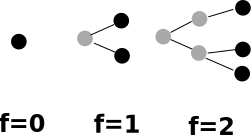
\includegraphics{img/trees.png}
 \caption{Figure depicting OpenTrees.}
 \label{trees}
\end{figure}

\subsection{Theoretical Analysis of OpenTrees}

An OpenTrees stochastically returns a state in a branch of the search tree with the least number of leaf nodes. Consider two nodes $n_1,n_2$ in \refig{probability}. These are directly generated from a parent node $n_p$ by different actions $a_1,a_2$. Their paths from the initial state only differs in this single step, in other words they share the very long path prefix. The probability of selecting the branch of $n_p$ is evenly shared by $n_1,n_2$ -- it becomes the half of selecting $n_p$. Thus, a path which have a longer prefix shared with another path has a smaller probability to be opened first (although they should be opened eventually when the current OpenTrees is exhausted), and OpenTrees returns the most surprizing node in terms of path difference.
This results in maximising the surprisal of the path that leads to the returned node.
% This results in returning a state which has the largest ``surprise'' in terms of the pathes that leads to the open nodes.

% \begin{figure}[htbp]
%  \centering
%  \relsize{-2}
%  \includegraphics{img/open-tree-probability.png}
%  \caption{The probability of each leaf node to be opened, along with the probability of the helper % nodes to be visited. The nodes in a branch already heavily expanded are selected in a smaller % possibility, and the nodes in a narrower branch gets the higher possibility. It thus manages the % diversity of the search.}
%  \label{probability}
% \end{figure}

The novelty of this algrithm compared to the previous RRT-A* combinations is that we adopted the edit distance of the paths instead of state distance e.g. plan distance or relaxed plan distance.
Comppared to the plan distance, path distance is very easy to compute. Also, OpenTree implicitly balances the diversity of the search avoiding the costly $O(n^2)$ Nearest Neighbor Search.

\subsection{Experimental Results}
\label{sec-3}

We conducted experiments on 3 tractable heuristic functions, blind, $h^{\mbox{max}}$ and Landmark Cut heuristics (LMcut) \cite{Helmert2009}, as well as the intractable heuristics such as almost perfect heuristics with $c=3$ and the perfect heuristics.

In evaluating our approach on tractable heuristic functions, we applied a standard competition settings of 30min.\ time limit and 2GB memory limit.

In the experiments simulating almost perfect heuristics and perfect
heuristics, time limit is not applied and the heuristic values are computed by searching
from the node to the goal using optimal planning with LMcut. Thus, the
problem instances used in these settings are limited to the small instances.

The coverage results in \reftbl{tbl:main} show that OpenTrees significantly improves upon \astar across the tractable functions, and also across the intractable functions. We also show that the number of expansions in OpenTrees is significantly smaller than that of \astar. Note that the number of expansion when the heuristic estimate is larger than zero is the same between these two algorithms.

%The implications here is that the diversity information is orthogonal to the information %obtained from the distance estimation. In intractable heuristics, we can assume nearly all %information from the domain, current state and the goal state is obtained because we cannot %improve upon perfect heuristics. The only remaining unexploited information is left in the %relationship between the search nodes.
{ \setlength{\tabcolsep}{0.1em}
\begin{table}[htbp]
\centering \relsize{-1}
\begin{tabular}{|l|ll|ll||ll|}
\hline
 & blind &  & LMcut &  & Almost & Perfect  \\
 &  &  &  &  & $c=3$ &   \\
Domains & \astar & OT & \astar & OT & \astar & OT  \\
\hline
Gripper(20) & 9 & 10 & 12 & \textbf{13} &  &   \\
Depot(20) & 11 & 11 & 15 & \textbf{20} &  &   \\
Airport(30) & \ldots{} &  &  &  &  &  \\
TPP &  &  &  &  &  &   \\
CyberSec &  &  &  &  &  & \\
Sokoban &  &  &  &  &  &  \\
\ldots{} &  &  &  &  &  &  \\
\ldots{} &  &  &  &  &  &  \\
\ldots{} &  &  &  &  &  &  \\
\ldots{} &  &  &  &  &  &  \\
\ldots{} &  &  &  &  &  &  \\
expected & wi & dth & and & hei & ght & \\
\ldots{} &  &  &  &  &  & \\
\ldots{} &  &  &  &  &  & \\
\ldots{} &  &  &  &  &  & \\
\ldots{} &  &  &  &  &  & \\
\ldots{} &  &  &  &  &  & \\
\ldots{} &  &  &  &  &  & \\
\ldots{} &  &  &  &  &  & \\
Zenotravel &  &  &  &  &  & \\
\hline
Total & 800 & \textbf{900} &  &  &  & \\
\hline
\end{tabular}
\caption{The coverage results of \astar and $^*A^*$ with 30 min experiments on 2 GB machine. Best results across the tractable heuristics are indicated in \textbf{bold}.}
\label{tbl:main}
\end{table}

}

In \refig{diversity-transition}, we plotted the transition of diversity in the plateau as the expansion continues. The $y$-axis, the diversity across the plateau, was computed according to the formula $D(S_o)=abc/def$ where $S_o$ is the set of states with the best f-value in the open list. The $x$-axis in the figure shows the ratio of the size of $S_o$ to the size of $S_c$, the set of states in the closed list with best f-value, indicating the search progress.

It shows that the diversity in the open list remains high in OpenTrees, while it quickly decreases in \astar. It indicates that the expansion is done evenly on various kinds of nodes, rather than in a biased manner that the expansion is focused on a particular set of nodes.
% \todo{of course, the real figure should not be an ASCII art!}

\begin{figure}[htbp]
\begin{verbatim}
LMcut          Almost Perfect       

D(S)             D(S)                             
|                |             
||\___OpenTrees  ||\___OpenTrees
|\    \____      |\    \____   
| \        \__   | \        \__
|  ~\ A*+FIFO    |  ~\ A*+FIFO 
|    ~-_______   |    ~-_______
+------------->  +------------->
      #(S_c)/#(S_o)     #(S_c)/#(S_o)
\end{verbatim}
\caption{Transition of the diversity in the unexpanded best-f nodes in the open list.}
\label{diversity-transition}
\end{figure}

\section{Related Work}
\label{sec-4}

\emph{Symmetry Breaking} \cite{Fox1998,pochter2011exploiting,domshlak2013symmetry} is the search technique that tries to prune the states with symmetric paths. \emph{Partial Order Reduction}, \emph{Strong Stubbern Sets} and \emph{Expansion Core} are also the techniques which prune the intermediate states that reach to the same goal using the different orders of same actions. \emph{Dominance Pruning} \cite{erol1994} is a technique which exploits additional information from the problem after the heuristics are computed. Instead of computing the absolute distance, it  proves if a state is strictly relatively better than the other nodes. Since path similarity is weaker than symmetry or other criteria, our approach does not prune states, and instead just delay the expansion within the same f-value.

The plan diversity research by \cite{goldman2015measuring} makes use of Normalized Compression Distance(NCD), which approximates Normalized Information Distance(NID), devised by Kolmogolov complexity theory and only semicomputable. NCD approximates NID by using a common or a \sota compression algorithms such as gzip, bzip or ppmz. NCD and NID are both the distance between the  \emph{strings}, and thus are suitable for computing the difference of paths. Edit distance in OpenTree is a much cheper approximation to NID.

One application of diversity-based technique is \emph{HTN} \cite{erol1994} and \emph{Factored Planning} \cite{amir2003factored,brafman2006factored,Asai2015}. Earlier work on diversity \cite{goldman2015measuring} proposed a method to choose the best set of learning targets of HTN learner based on diversity. Similar method could be applied to choose the best set of factors in the framework.


\section{Conclusion}

In this paper, we proposed two novel diversity-aware tie-braking methods for the admissible search using \astar. We empirically showed that they improve the performance on various domains, and they are heuristic-agnostic improvements. We showed that they have a significant impact on the final step of the search in large plateau.
 % when the distribution of optimal solutions is not uniform within the open list.
% We also showed that this nonuniform distribution still appears when we have almost-perfect % heuristics.
Our method differs from the other pruning techniques such as symmetry breaking, dominance pruning or partial-order-pruning because we actually do not prune any states, nor from the other general improvements in the heuristic accuracy because we just change the expansion order within the same $f$.

Although the diversification of the planning algorithms has a large interest driven by the practical applications, research on the performance improvement with diversity has long been neglected, especially in admissible search. This paper specifically addresses this issue. We also  contribute to the planning community by proposing the maximum scope of information that can be exploited when we have almost perfect heuristics. This, for example, may provide an observation that some of the information in symmetry or dominance pruning might be already captured by the almost-perfect heuristics, while others are not. This distinction of the goal-directed information and the past information may be helpful on designing and understanding the new types of future planning algorithms.

